\documentclass[a4paper]{article}

\usepackage[utf8]{inputenc}
\usepackage[portuges]{babel}
\usepackage{a4wide}
\usepackage{multicol}
\usepackage{spverbatim}
\usepackage{graphicx}

\title{Projeto de LI3 - Wikipedia\\Grupo 69}
\author{Sérgio Jorge (A77730) \and Vítor Castro (A77870) \and Marcos Pereira (A79116)}
\date{}


\begin{document}

\maketitle

\begin{abstract}
Neste relatório faremos uma análise do primeiro projeto de Laboratórios de Informática III, cujo objetivo era desenvolver um programa, na linguagem de programação C, que fizesse a leitura de \textit{backups} em XML da \textit{Wikipedia}, respondendo a diversas interrogações propostas. Assim, este documento apresenta detalhadamente a abordagem tomada, quer na sua generalidade, quer ao nível das interrogações individuais.
\end{abstract}

\tableofcontents

\section{Introdução}
\label{sec:intro}
Este projeto foi realizado com o objetivo de construir um programa capaz de fazer uma análise dos artigos que estão nos \textit{backups} da \textit{Wikipedia} fornecidos pela equipa docente, para que seja possível determinar informações úteis acerca desses mesmos \textit{backups}.
Assim, foram propostas pelos professores 10 tarefas computacionais, às quais o nosso programa, construído em C, deverá responder com sucesso. A realização das 10 tarefas permitiram, por um lado, melhorar e consolidar os conhecimentos adquiridos nas UCs de Programação Imperativa, Algoritmos e Complexidade e Arquitetura de Computadores. Por outro, incentivaram à exploração de bibliotecas como a \textit{libxml2} e a \textit{GLib}, enquanto desafiaram à modularidade estritamente necessária para a participação capaz no desenvolvimento em grupo de um projeto como este.
Dado o tamanho dos \textit{backups} e da necessidade de fazer procuras rápidas, só \textit{hashtables} fizeram sentido, pelo que é com elas que vamos fazer todo o armazenamento de dados.
Assim, de modo a facilitar a compreensão do projeto, o relatório está dividido da seguinte forma:
\begin{description}
    \item[Secção 2 :] Problema;
    \item[Secção 3 :] Solução;
    \item[Secção 4 :] Conclusão.
\end{description}

\section{Problema}
\label{sec:problema}
Neste projeto de LI3, é-nos pedido para a partir de \textit{backups} da \textit{Wikipedia}, fornecidos pelos professores, fazermos a leitura dos dados e a extração de informação que a equipa docente considera relevante. Assim, a informação que devemos gerar é:
\begin{description}
\item[1 - All articles]\hfill \\
devolver o número de artigos analisados nos \textit{backups}.
\item[2 - Unique articles]\hfill \\
devolver o número de artigos únicos (com ID único) encontrados nos vários \textit{backups} analisados.
\item[3 - All revisions]\hfill \\
devolver quantas revisões foram efetuadas nos \textit{backups}.
\item[4 - Top 10 contributors]\hfill \\
devolver um \textit{array} com os identificadores dos 10 autores que mais contribuíram, quer em artigos únicos, quer em revisões de artigos já existentes. O resultado deve ser ordenado pelos autores com mais contribuições, sendo que se existirem autores com o mesmo número de contribuições, o resultado deve apresentar primeiro os autores com um identificador menor.
\item[5 - Contributor name]\hfill \\
devolver o nome do autor com um determinado identificador, ou \textbf{NULL} caso não exista.
\item[6 - Top 20 largest articles]\hfill \\
devolver um \textit{array} com os identificadores dos 20 artigos que possuem textos com um maior tamanho em bytes. Para cada artigo deve ser contabilizado o maior texto encontrado nas diversas versões (revisões) do mesmo. O resultado deve ser ordenado pelos artigos com maior tamanho. Se existirem artigos com o mesmo tamanho, o resultado deve apresentar primeiro os artigos com um identificador menor.
\item[7 - Article title]\hfill \\
devolver o título do artigo com um determinado identificador, ou \textbf{NULL} caso não exista.
\item[8 - Top N articles with more words]\hfill \\
devolver um \textit{array} com os identificadores dos N (passado como argumento) artigos que possuem textos com o maior número de palavras e o resultado deve ser ordenado pelos artigos com maior número de palavras.
\item[9 - Titles with prefix]\hfill \\
devolver um \textit{array} de títulos de artigos que começam com um prefixo passado como argumento e o resultado deve ser ordenado por ordem alfabética, ou \textbf{NULL} caso não existam artigos com esse prefixo.
\item[10 - Article timestamp]\hfill \\
devolver o \textit{timestamp} para uma certa revisão de um artigo, ou \textbf{NULL} caso não haja essa revisão.
\end{description}

\section{Solução}
A nossa solução foi implementada com base em diferentes módulos dos quais destacamos os quatro principais:

\begin{itemize}
    \item Parser
    \item Hashtable
    \item Users
    \item Articles
\end{itemize}
\label{sec:solucao}

\subsection{Parser}
Módulo que funciona com base na biblioteca \textit{libxml2}. A \textit{libxml2} é uma biblioteca para a linguagem C que nos permite trabalhar com ficheiros .xml e, em específico para o trabalho, percorrer o ficheiro de nodo em nodo, retirando o seus conteúdos ou tratando-os de forma útil.
Assim, é-nos então possível percorrer o ficheiro, iterar pelas páginas, e fazer o parse extraindo elementos como: \textit{Title}, \textit{ID} e \textit{Revision} (a cada \textit{Revision} está associado: \textit{ID}, \textit{ParentID}, \textit{Timestamp}, \textit{ContributorID}, \textit{ContributorUsername}, \textit{Text}).
A informação vai sendo transferida para a memória, que se concretiza na forma de \textit{hashtables} criadas com a \textit{GLib}, estrutura que a seguir invocamos.

\subsection{Hashtables}
Módulo que atráves do uso da biblioteca \textit{GLib}, armazena os dados transmitidos pelo \textit{parser}. Optamos pela uso de 2 hashtables principais (\textit{articles} e \textit{users}), sendo que a primeira tem uma \textit{hashtables revisions} para cada artigo.
\begin{description}
    \item[Hashtable \textit{articles}] Esta tabela armazena a ID de cada artigo, o tamanho do texto em \textit{bytes}, o número de palavras do texto, o título, e além disso cria, caso o artigo não exista ainda, uma \textit{hashtables revisions} onde é inserida informação relativamente à revisão que está a ser processada.

    \item[Hashtable \textit{revisions}] Cada artigo tem a ele associado uma estrutura de dados deste tipo com as revisões.

    \item[Hashtable \textit{users}] Esta estrutura de dados armazena o ID de cada contribuidor, o \textit{username} do contribuidor e o seu número de contribuições.

\end{description}

\subsection{Users}
 Este módulo trata de calcular as respostas a todas as \textit{queries} relativas aos contribuidores, fazendo uso das \textit{hashtables} já preenchidas. Além disso, faz a ligação entre o módulo \textbf{\textit{Parser}} e o módulo \textbf{\textit{Hashtable}}, processando toda a informação obtida no \textit{parsing} e enviando para a \textit{hashtable users} apenas informação relevante.

\subsection{Articles}
 Muito semelhante ao \textbf{\textit{Users}}, este módulo trata de calcular as respostas a todas as queries relativas aos artigos, fazendo uso das \textit{hashtable} de artigos e da \textit{hashtable} de revisões presente em cada entrada da anterior. Faz também a ligação entre o módulo \textbf{\textit{Parser}} e o módulo \textbf{\textit{Hashtable}} aquando do parse inicial dos dados, passando também apenas a informação relevante para as \textit{hashtables articles} e \textit{revisions}.

\subsection{Implementação}

\subsubsection{All articles, Unique articles e All revisions}
Para resolvermos estas interrogações, optamos por utilizar dois pointers (\textit{articleWasFound} e \textit{articleWasUpdated}), que são alterados em runtime quando se decide que campos das hashtable são criados ou alterados.
Assim, sempre que se recebe um artigo, verifica-se se este já existe na estrutura de dados:
Se não existe, \textit{articleWasFound} = 0 e \textit{articleWasUpdated} = 1 e, cria o novo artigo na hashtable de artigos, cria a hashtable de revisões e adiciona a revisão à hashtable de revisões. Apesar de não ser encontrado o artigo, é feito o update do mesmo, o que nos permite aumentar o contador allRevisions, presente na \textit{hashtables articles}.
Se o artigo já existe na estrutura de dados, \textit{articleWasFound} = 1 e verifica-se o que surgiu de diferente no artigo. Então, se de facto surgiram alterações ao artigo, \textit{articleWasUpdated} = 1. Senão, \textit{articleWasUpdated} = 0. Além disso, a revisão é introduzida na hashtable de revisões do artigo em questão, caso o artigo tenha algo diferente. Neste caso, em que adicionamos um novo artigo à tabela, incrementamos o contador uniqueArticles, presente na \textit{hashtables articles}.
Portanto, \textbf{\textit{All articles}} é alcançado a partir de um contador que é incrementado sempre que é encontrado um artigo, independentemente dos apontadores \textit{articleWasFound} e \textit{articleWasUpdated}. \textbf{\textit{Unique articles}} é devolvido a partir de um contador que é incrementado se e só se o \textit{articleWasFound} está com valor 0. \textbf{\textit{All revisions}} é calculado também a partir de um contador que é incrementado quando o \textit{articleWasUpdated} = 1.
Termos estes contadores na \textit{hashtable} foi a maneira que nos pareceu mais eficiente de colher tais informações, uma vez que o custo seria apenas de mudar o valor de um apontador, contrariamente ao que seria o custo de, por exemplo, percorrer toda a \textit{hashtable} no fim e incrementar os mesmos contadores.

\subsubsection{Top 10 contributors}
Definimos um \textit{array} com 10 posições para colocar o top. Percorremos a \textit{hashtable} de utilizadores e, para cada user, vamos buscar o seu número de contribuições e comparamos se tem mais que o utilizador que está na última posição do top (índice 9). Em caso afirmativo, comparamos com as sucessivas posições, encontramos a posição e deslizamos o resto dos utilizadores para haver lugar para o que está a ser tratado. Para os casos em que temos igual número de contribuições na comparação, faz-se a comparação dos ID dos users para sabermos qual o com menor ID.
Escolhemos fazer a comparação sempre pelo último lugar do top pois evitamos que, na maioria das vezes, se percorra o top sem necessidade.

\subsubsection{Contributor name}
É feita a procura passando o ID a uma função getUser do módulo hashtable que, caso exista tal ID na \textit{hashtable users}, retorna uma estrutura de utilizador com todos os dados correspondentes àquele utilizador em específico. Caso não exista, retorna \textbf{NULL}. Depois, é feito o acesso ao campo username daquele user, na função \textbf{getContributorName} do módulo \textbf{\textit{Users}}.

\subsubsection{Top 20 largest articles}
Definimos um \textit{array} com 20 posições para colocar o top. Percorremos a \textit{hashtable} de artigos e, para cada artigo, vamos buscar o número do texto em bytes e comparamos se tem mais que o artigo que está na última posição do top (índice 19). Em caso afirmativo, comparamos com as sucessivas posições, encontramos a posição e deslizamos o resto dos artigos para haver lugar para o autal. Para os casos em que temos igual número de contribuições na comparação, faz-se uma compaação dos IDs dos articles para sabermos qual o menor ID.
Tal como na solução \textbf{Top 10 contributors}, fizemos a comparação a partir do último elemento do top.
O tamanho em bytes é obtido através da função \textbf{wordCounter}, presente em articles, que atualiza um pointer com o valor do tamanho da \textit{string} analisada. Em \textbf{Top N articles with more words} explica-se um pouco melhor esta função.

\subsubsection{Article title}
É feita a procura passando o ID a uma função \textbf{getArticle} do módulo \textit{hashtable} que, caso exista tal ID na \textit{hashtable articles}, retorna uma estrutura de artigo com todos os dados correspondentes àquele artigo em específico. Caso não exista, retorna \textbf{NULL}. Depois, é feito o acesso ao campo \textit{title} daquele \textit{article}, na função \textbf{get\_article\_title} do módulo articles.

\subsubsection{Top N articles with more words}
Definimos um \textit{array} com n posições para colocar o top. Percorremos a \textit{hashtable} de artigos e, para cada artigo, vamos buscar o número de palavras e comparamos se tem mais que o artigo que está na última posição do top (índice n-1). Em caso afirmativo, comparamos com as sucessivas posições, encontramos a posição e deslizamos o resto dos artigos para haver lugar para o atual. Para os casos em que temos igual número de contribuições na comparação, faz-se um string compare dos dois ID dos articles para sabermos qual o menor ID.
Faz-se a comparação a partir do último lugar do top pelos mesmos motivos que em \textbf{Top 10 contributors} e em \textbf{Top 20 largest articles}.
Para ver o número de words usou-se a função \textbf{wordCounter}, do módulo \textit{articles}, que tinha \textit{flags} para que fosse possível controlar os espaços entre palavras e carateres especiais, de modo a que se obtivesse números fiáveis. O contador usado para avançar de char em char é também usado para fornecer, no final, o número total de \textit{bytes} do artigo, o que resulta num poupar de trabalho significativo, sendo esta função uma 2 em 1 que também é importante no \textbf{Top 20 largest articles}.

\subsubsection{Titles with prefix}
A forma que encontramos para resolver este problema foi implementar a função \textbf{isTitlePrefix} que verifica se determinada \textit{string} é prefixo de outra \textit{string}. Assim, percorremos a \textit{hashtable} de artigos e chamamos a função implementada e verificamos se os títulos são prefixo. Em caso afirmativo, inserimos o título num \textit{array} definido para o efeito de armazenar todos os títulos com o prefixo dado como argumento. Posteriormente, o \textit{array} de títulos é ordenado por ordem alfabética.

\subsubsection{Article timestamp}
É feita a procura passando o ID a uma função getArticle do módulo \textit{hashtable} que, caso exista tal ID na \textit{hashtable articles}, retorna uma estrutura de artigo com todos os dados correspondentes àquele artigo em específico. Caso não exista, retorna \textbf{NULL}. Depois, é feito o acesso ao campo \textit{timestamp} daquele \textit{article}, na função \textbf{get\_article\_timestamp} do módulo \textbf{\textit{Articles}}.

\pagebreak
\subsection{Resultado Final}

\begin{figure}[htbp]
    \centering
    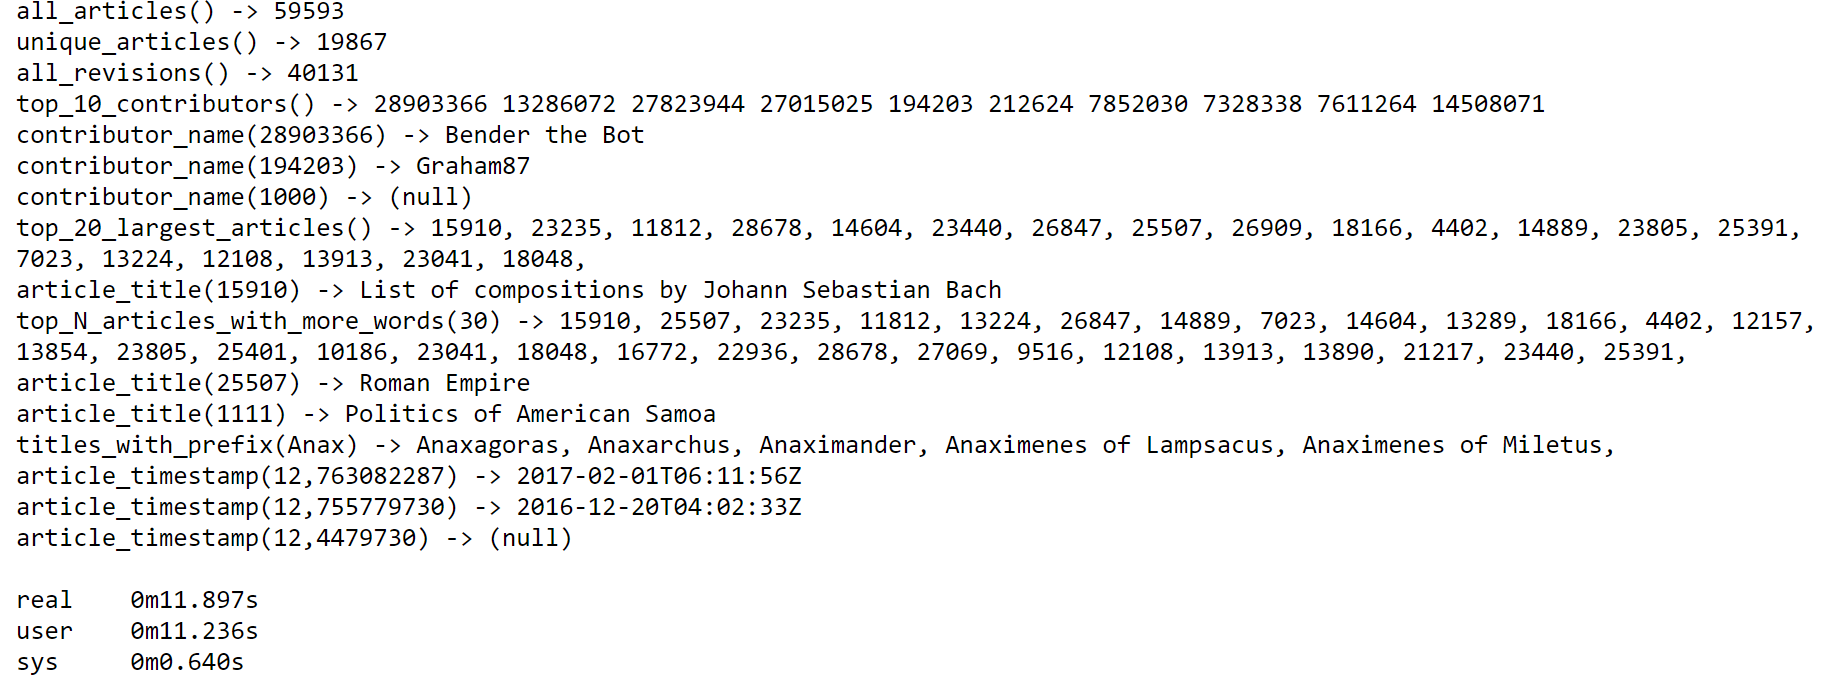
\includegraphics[width = 420pt, height = 230pt]{output}
\end{figure}

\section{Conclusões}
\label{sec:conclusao}
Este projeto serviu para aprofundarmos o conhecimento da linguagem C, assim como as bibliotecas que lhe estão associadas. Achámos que, com a realização de um trabalho deste tipo permite uma consolidação proveitosa da linguagem, não só em termos teóricos como também em termos práticos e acaba por ser uma forma diferente de cimentar os conteúdos de algumas das UCs que nos surgiram neste curso. Permite também melhorar as habilidades na resolução de problemas. Concluímos também que:

\begin{itemize}
        \item O uso da estrutura de dados adequada (\textit{hashtables}) foi essencial de forma a obter um programa eficiente, que faça a manipulação necessária dos dados em tempo útil;
 	    \item A separação do trabalho em módulos permite uma fácil divisão do trabalho pela equipa, aliando-se ao uso do \textbf{\textit{Git}} numa organização eficiente do trabalho do grupo.
\end{itemize}

\end{document}